\documentclass[aps,superscriptaddress,tightenlines,nofootinbib,floatfix,longbibliography,notitlepage]{revtex4-1}
\usepackage[left=18mm,right=19mm,top=23mm,bottom=16mm]{geometry}
\usepackage{amsmath,amssymb}
\usepackage{bm}
\usepackage{comment}
\usepackage{graphicx}
\usepackage[dvipsnames]{xcolor}
\usepackage{slashed}
\usepackage[
    colorlinks=true,
    allcolors=blue
]{hyperref}

\newcommand\todo[1]{{\bf\color{red}TODO: #1}}

%%%
%%%     Incorporate Repository Information
%%%

\providecommand{\repositoryInformationSetup}{} % Fallback definition if not compiled with `make DRAFT=1`.
\repositoryInformationSetup

%%%
%%%     Include latex-base macros
%%%

\usepackage{xspace}
\usepackage{bbm}

%%%%
%%%%    Project Specifics
%%%%
\newcommand{\Luscher}{L\"{u}scher\xspace}
% \newcommand{\nstep}{\ensuremath{{n_\text{step}}}\xspace}
\newcommand{\nstep}{\ensuremath{{n_s}}\xspace}
\newcommand{\spherical}{\ensuremath{\bigcirc}\xspace}
\newcommand{\cartesian}{\ensuremath{\square}\xspace}
\newcommand{\counterterm}{\ensuremath{\mathcal{L}}}
\newcommand{\dispersion}{\ensuremath{\boxplus}\xspace}
% \newcommand{\dispersion}{\ensuremath{\sharp}\xspace}
\newcommand{\PV}{\ensuremath{\mathcal{P}}}
\newcommand{\normalization}{\ensuremath{\mathcal{N}}\xspace}

\newcommand{\lowEnergyA}{\ensuremath{\mathcal{A}}}
\newcommand{\F}{\ensuremath{\mathcal{F}}}
\newcommand{\FV}{\ensuremath{\textrm{FV}}}
\newcommand{\xtilde}{\ensuremath{\tilde{x}}\xspace}
\newcommand{\Aoneg}{\ensuremath{A_{1g}}\xspace}
\renewcommand{\l}{\ensuremath{\ell}\xspace}
\newcommand{\Laplacian}{\ensuremath{\mathop{}\!\mathbin\bigtriangleup}}
\newcommand{\BZ}{\text{B.Z.}}

%%%%
%%%%    Referring to Parts of the Repo
%%%%
\newcommand{\repoURL}{https://github.com/ckoerber/luescher-nd}
\newcommand{\issue}[1]{\href{\repoURL/issues/#1}{Issue #1}}
\newcommand{\pullrequest}[1]{\href{\repoURL/pulls/#1}{Pull Request #1}}

%%%%
%%%%    Referring to Parts of the Document
%%%%
\newcommand{\secref}[1]{Sec.~\ref{sec:#1}}
\newcommand{\Secref}[1]{Section~\ref{sec:#1}}
\newcommand{\appref}[1]{App.~\ref{sec:#1}}
\newcommand{\Appref}[1]{Appendix~\ref{sec:#1}}
\newcommand{\tabref}[1]{Tab.~\ref{tab:#1}\xspace}
\newcommand{\Tabref}[1]{Table~\ref{tab:#1}\xspace}
\newcommand{\figref}[1]{Fig.~\ref{fig:#1}\xspace}
\newcommand{\Figref}[1]{Figure~\ref{fig:#1}\xspace}
\renewcommand{\eqref}[1]{(\ref{eq:#1})\xspace}
\newcommand{\Eqref}[1]{Equation~\ref{eq:#1}\xspace}
\newcommand{\Ref}[1]{Ref.~\cite{#1}}
\newcommand{\Reference}[1]{Reference~\cite{#1}}
\newcommand{\Refs}[1]{Refs.~\cite{#1}}
\newcommand{\References}[1]{References~\cite{#1}}
%%%%
%%%%    Referring to Other Documents
%%%%

\renewcommand{\doi}[1]{\href{http://doi.org/#1}{[#1]}}
\newcommand{\arxiv}[1]{\href{http://www.arxiv.org/abs/#1}{arXiv:#1}}

%%%%
%%%%    Mathematical Symbols
%%%%

\newcommand{\goesto}{\ensuremath{\rightarrow}}
\newcommand{\infinity}{\infty}
\newcommand{\Integers}{\mathbb{Z}\xspace}
\newcommand{\integers}{\Integers}
\newcommand{\one}{\ensuremath{\mathbbm{1}}}
\newcommand{\order}[1]{\ensuremath{\mathcal{O}\left(#1\right)}\xspace}
\newcommand{\Rationals}{\mathbb{Q}\xspace}
\newcommand{\Reals}{\mathbb{R}\xspace}
\newcommand{\union}{\ensuremath{\cup}}
\DeclareMathOperator{\erf}{erf}
\DeclareMathOperator{\erfi}{erfi}
\renewcommand{\mod}[1]{\ensuremath{\ \left(\text{mod }#1\right)}}

%%%%
%%%%    Hyperbolic Trig
%%%%

% Most are already available if you \usepackage{amsmath}.
% However, those below are missing

\DeclareMathOperator{\sech}{sech}
\DeclareMathOperator{\csch}{csch}
\DeclareMathOperator{\arccosh}{arccosh}
\DeclareMathOperator{\arcsinh}{arcsinh}
\DeclareMathOperator{\arctanh}{arctanh}
\DeclareMathOperator{\arcsech}{arcsech}
\DeclareMathOperator{\arccsch}{arccsch}
\DeclareMathOperator{\arccoth}{arccoth}

% Additionally, there are some missing trig functions:

\DeclareMathOperator{\arcsec}{arcsec}
\DeclareMathOperator{\arccot}{arccot}
\DeclareMathOperator{\arccsc}{arccsc}

%%%%
%%%%    Fractions
%%%%

\newcommand{\oneover}[1]{\ensuremath{\frac{1}{#1}}}                             %   1/[argument]
\newcommand{\inverse}{\ensuremath{^{-1}}}                                       %   argument^-1
\newcommand{\half}{\ensuremath{\frac{1}{2}} }                                   %   1/2
\newcommand{\quarter}{\ensuremath{\frac{1}{4}} }                                %   1/4


%%%%
%%%%    Mathematical Delimiters
%%%%
\newcommand{\abs}[1]{\ensuremath{\left| #1 \right|}\xspace}
\newcommand{\magnitude}{\abs}
\newcommand{\average}[1]{\ensuremath{\left\langle #1 \right\rangle}\xspace}

% Quantum mechanics bra-ket notation:
\newcommand{\ket}[1]{\ensuremath{\left|\;#1\;\right\rangle}}
\newcommand{\bra}[1]{\ensuremath{\left\langle\;#1\;\right|}}
\newcommand{\bracket}[2]{\ensuremath{\left\langle\;#1\;\middle|\;#2\;\right\rangle}}
\let\braket\bracket
\newcommand{\braMket}[3]{\ensuremath{\left\langle\;#1\;\middle|\;#2\;\middle|\;#3\;\right\rangle}}


%%%%
%%%%    Matrices
%%%%

\newcommand{\identity}{\ensuremath{\mathds{1}}}
\newcommand{\diag}[1]{\ensuremath{\text{diag}\left(#1\right)}}
\newcommand{\tr}[1]{\ensuremath{\text{tr}\left[#1\right]}}
\newcommand{\transpose}{\ensuremath{{}^{\top}}}

%%%%
%%%%    Physical Quantities and Constants
%%%%




%%%%
%%%%    Software
%%%%

\newcommand{\bash}{\texttt{bash}\xspace}
\newcommand{\git}{\texttt{git}\xspace}
\newcommand{\make}{\texttt{make}\xspace}
\newcommand{\mpi}{\texttt{MPI}\xspace}
\newcommand{\python}{\texttt{python}\xspace}

% Put an xspace after \LaTeX:
\let\builtinLaTeX\LaTeX
\def\LaTeX{\builtinLaTeX\xspace}
 % input rather than include so we don't create macros.aux

%%%%
%%%%    Document preparation
%%%%

\begin{document}

\title{Don't Cut Corners when Deriving L\"{u}scher's Formula}
\newcommand{\ikp}{
    Institut f\"{u}r Kernphysik,
    Forschungszentrum J\"{u}lich, 54245 J\"{u}lich Germany
}

\newcommand{\ias}{
    Institute for Advanced Simulation,
    Forschungszentrum J\"{u}lich, 54245 J\"{u}lich Germany
}

\newcommand{\julich}{
    Institut f\"{u}r Kernphysik and Institute for Advanced Simulation,
    Forschungszentrum J\"{u}lich, 54245 J\"{u}lich Germany
}

\newcommand{\bonn}{
    Helmholtz-Institut f\"{u}r Strahlen- und Kernphysik,
    Rheinische Friedrich-Wilhelms-Universit\"{a}t Bonn, 53012 Bonn Germany
}

\newcommand{\jsc}{
    J\"{u}lich Supercomputing Center,
    Forschungszentrum J\"{u}lich, 54245 J\"{u}lich Germany
}

\newcommand{\berkeley}{
    Department of Physics,
    University of California, Berkeley, CA 94720, USA
}

\newcommand{\lbnl}{
    Nuclear Science Division,
    Lawrence Berkeley National Laboratory, Berkeley, CA 94720, USA
}

\newcommand{\umd}{
    Department of Physics,
    University of Maryland, College Park, MD 20742,
    USA
}

\newcommand{\mcfp}{
    Maryland Center for Fundamental Physics,
    University of Maryland, College Park, MD 20742,
    USA
}

\author{Christopher K\"orber}   \affiliation{\berkeley} \affiliation{\lbnl}
\author{Evan Berkowitz}         \affiliation{\julich} \affiliation{\mcfp}
\author{Thomas Luu}             \affiliation{\julich} \affiliation{\bonn}





\date{\today}

\begin{abstract}
L\"{u}scher's generalized zeta functions, encountered when translating finite-volume spectra into infinite-volume phase shifts, are sums typically over a momentum whose magnitude is cut off and regularized using a spherical integral.  By exactly solving two-body quantum mechanical problems we show that the correct procedure is to formulate these functions so that they match the procedure executed when taking the continuum limit, so that in a cubic volume the entirety of the Brillouin zone is accounted for, changing the counter term.
\todo{Also we are smart in other ways.  Dispersion etc.}
\end{abstract}

\maketitle

\section{Introduction}\label{sec:intro}

\todo{We should start with focussing on unitarity.}

\Luscher's finite-volume formalism\cite{Hamber198399,luscher:1986I,luscher:1986II,wiese1989,Luscher1991,Luscher1991237} is the method by which we can extract infinite-volume real-time scattering data from the finite-volume Euclidean spectrum of a theory, taking advantage of the interplay between the physical scattering and the finite-volume boundary conditions in determining the spectrum.

The usual understanding of \Luscher's formalism is that one should find the continuum zero-temperature finite-volume energy levels, holding the physical volume fixed, and put that cold, continuum spectrum through \Luscher's formula to extract continuum scattering data.

In practice, few results of lattice QCD calculations are zero-temperature- or, more seriously, continuum-extrapolated, but are nevertheless put through \Luscher's formula to get an estimate of the continuum scattering data, assuming thermal and discretization effects to be much smaller than the statistical uncertainties\todo{cite cite cite}.
In particular, no continuum-limit study of any baryonic channel exists, even at physically heavy pion masses.

While alternatives, including the potential method (see, for example \Refs{Ishii:2006ec,Nemura:2008sp,Aoki:2009ji,Murano:2011nz,Aoki:2012bb,Kurth:2013tua,Sugiura:2017vwo,Yamazaki:2019vid,Aoki:2017yru,Yamazaki:2018qut,Iritani:2017rlk,Iritani:2018zbt,Gongyo:2018gou,Akahoshi:2019klc,Namekawa:2019xiy}) and the imposition of spherical walls\cite{Borasoy:2007vy,Borasoy:2007vi,Lee:2008fa,Epelbaum:2008vj,Epelbaum:2010xt,Elhatisari:2015iga,Elhatisari:2016owd,Elhatisari:2016hby,Klein:2018lqz,Li:2019ldq,Bovermann:2019jbt}, can be used to translate finite-volume physics to infinite-volume observables we focus here on the \Luscher finite-volume formalism.

Here, we construct example Hamiltonians explicitly and diagonalize them exactly.
This allows us to circumvent all of the issues of statistical uncertainty that accompanies Monte Carlo data, and lets us completely isolate the features of the formalism itself, removing, for example, any finite-temperature effects that should in principle be extrapolated away in any finite-temperature method like Lattice QCD.

We find that it is actually quite difficult to reliably extrapolate the spectrum to the continuum limit in a way that reproduces the exact known result, but that taking the continuum limit of the lattice-artifact-contaminated phase shifts seems to produce a more reliable result.
We also explain how to incorporate lattice artifacts into \Luscher's formula, accounting both for the Brillouin zone of the cubic lattice and the lattice-induced dispersion relation.

This lattice improvement can be quite useful.
In pursuit of a lattice formulation of unitary fermions, the authors of \Ref{Endres:2011er} followed the tuning procedure of \Ref{Lee:2007ae}, parametrizing the contact interaction as a sum of a tower of Galilean-invariant operators, tuning their coefficients so as to drive the lowest interacting energy levels to the zeros of the \Luscher finite-volume zeta function.
However, in \Ref{Endres:2012cw} they found that even with a highly-improved construction the states ultimately deviated from a $\pi/2$ phase shift (see, for example, Figure 3).
We introduce a new continuum-limit prescription for achieving unitarity in lattice simulations by tuning just the simplest contact operator, but taking the discretization effects into account by incorporating the lattice dispersion relation into the finite-volume zeta function, both in the tuning step and in the analysis step.
By re-tuning the interaction at each lattice spacing we can very easily and smoothly take the continuum limit after applying the lattice-aware finite-volume formula.
We demonstrate that this allows us to maintain a constant phase shift deep into the spectrum\todo{, in some cases covering as many \Aoneg states exist in the lattice of interest?}

This paper is organized as follow.  In \Secref{hamiltonian} we give specifics about the latticized contact-interaction Hamiltonians we study.  In \Secref{spherical} we use show that taking a fixed-volume continuum limit with the interaction strength tuned to reproduce the first zero of the traditional zeta function does not yield the expected flat effective range expansion.  In \Secref{cartesian} we reformulate the standard generalized zeta function with integrals defined over the (cubic) Brillouin zone of the lattice.
In \Secref{dispersion} we explain how to incorporate the single-particle dispersion relation into the \Luscher construction, and show that we can use such a relation to circumvent the need for a continuum limit spectrum in the unitary case.
We relegate the computation of the various finite-volume counterterms to the Appendix.

\section{Discretized Hamiltonian}\label{sec:hamiltonian}

We study the simplest interacting two-body problem, two particles interacting via a contact interaction,
\begin{equation}
    \label{eq:particle hamiltonian}
    H = \frac{p_1^2}{2 m_1} + \frac{p_2^2}{2 m_2} + C \delta(x_1-x_2)
\end{equation}
where the subscripts indicate the position of the position and momenta.  Moving to center-of-mass and relative coordinates, this becomes
\begin{equation}
    \label{eq:hamiltonian}
    H = \frac{P^2}{2 M} + \frac{p^2}{2 \mu} + C \delta(x)
\end{equation}
where capital letters represent center-of-mass variables, lower case implies relative coordinates, and $\mu$ is the reduced mass.  We henceforth specialize to the rest frame, setting $P=0$, which reduces the problem to an effective one-body problem.

We consider a finite cubic volume of linear size $L$ with periodic boundary conditions and lattice spacing $\epsilon$ so that $N=L/\epsilon$ is an even integer that counts the number of sites in one spatial direction.

On the lattice we implement the contact interaction as entirely local, vanishing everywhere except at the origin where it is of strength $C$.  We study a variety of kinetic operators, in contrast.  We denote the symmetric nearest-neighbor finite difference $\nstep=1$.  We consider additional stencils which extend on-axis additional steps so that the finite difference is a $(1+2\nstep D)$-point stencil in $D$ dimensions,
\begin{equation}
    \left\langle \vec{r}' \middle| H \middle| \vec{r} \right\rangle
    \rightarrow
    H_{\vec{r}',\vec{r}}^{(L,\epsilon,\nstep)}
    = - \frac{1}{2 \mu \epsilon^2} \sum_{d=1}^{D} \sum_{s=-\nstep}^{+\nstep} c^{(\nstep)}_{|s|} \delta_{\vec{r}',\vec{r}+\epsilon s \vec{e}_d} + C(\epsilon) \delta_{\vec{r}',\vec{r}}\delta_{\vec{r},\vec{0}}
\end{equation}
where the indices are understood to be modded by the periodic boundary conditions of the lattice.
In momentum space, this Hamiltonian may be written
\begin{align}
    \label{eq:p space hamiltonian}
    \left\langle \vec{p}' \middle| H \middle| \vec{p} \right\rangle
    \rightarrow
    H_{\vec{p}',\vec{p}}^{(L,\epsilon,\nstep)}
    &= \delta_{\vec{p}',\vec{p}} \frac{1}{2\mu} \sum_{d=1}^{D} \omega^{(\nstep)}(p_d,\epsilon) + C(\epsilon)
    \\
    \label{eq:gamma definition}
    \omega^{(\nstep)}(p_d,\epsilon)
    &= \frac{1}{\epsilon^2} \sum_{s=0}^{\nstep} \gamma_{s}^{(\nstep)} \cos(s p_d \epsilon)
\end{align}
where $\vec{p} = 2\pi \vec{n}/L$ for a $D$-plet of integers $\vec{n} \in (-N/2, +N/2]^D$, and the coefficients $\gamma_{s}^{(\nstep)}$ are determined by requiring the dispersion relation be as quadratic as possible,
\begin{equation}
    \label{eq:gamma determination}
    \omega^{(\nstep)}(p_d,\epsilon) \overset{!}{=} p_d^2 \left[ 1 + \order{(\epsilon p_d)^{2\nstep}}\right].
\end{equation}
In \Appref{coefficients} we collect the required $\gamma$ coefficients for a variety of $\nstep$s, and we show the resulting dispersion relations in \Figref{dispersion relation}.
In addition, we use a nonlocal operator, denoted by $\nstep=\infty$ which, in momentum space can be implemented to multiplying by $p^2$ directly,
\begin{equation}
    \omega^{\infty}(p_d,\epsilon) = p_d^2,
\end{equation}
including at the edge of the Brillouin zone, the Laplacian implementation of the ungauged SLAC derivative.
Including the edge does not introduce a discontinuity at the boundary (though it does introduce a cusp).

Once constructed, we diagonalize this Hamiltonian exactly to extract eigenenergies.
Throughout we focus on a three-dimensional system, though in \Appref{two-d} we study a two-dimensional system, where logarithmic divergences warrant special attention.

\begin{figure}
    \includegraphics[width=0.5\textwidth]{figure/dispersion.pdf}
    \caption{We show the continuum dispersion relation of energy as a function of momentum for different one-dimensional $\nstep$ derivatives.  For a finite number of lattice points $N$, the allowed momenta are evenly-spaced in steps of $2\pi/N$.
    As additional steps are incorporated into the finite difference, the dispersion relation more and more faithfully reproduces the desired $p^2$~behavior of $\nstep=\infty$.
    }
    \label{fig:dispersion relation}
\end{figure}

\section{The Usual, Spherical \Luscher's Formula}\label{sec:spherical}


Here we present a $D$-dimensional derivation of \Luscher's formula that roughly follows \Ref{Beane:2003da}, although the technology and sophistication of the finite-volume formalism has grown substantially \todo{cite cite cite}.  Assuming an interaction given by an tower of derivative contact operators
\begin{equation}
    V(p) = +\sum_n C_{2n}(\Lambda) p^{2n}
\end{equation}
where the interaction strengths depend on the regulator and carry spatial-dimension-dependent units.
The scattering amplitude is given by the bubble sum depicted in \Figref{bubbleSum}.

\begin{figure}[ht!]
\center
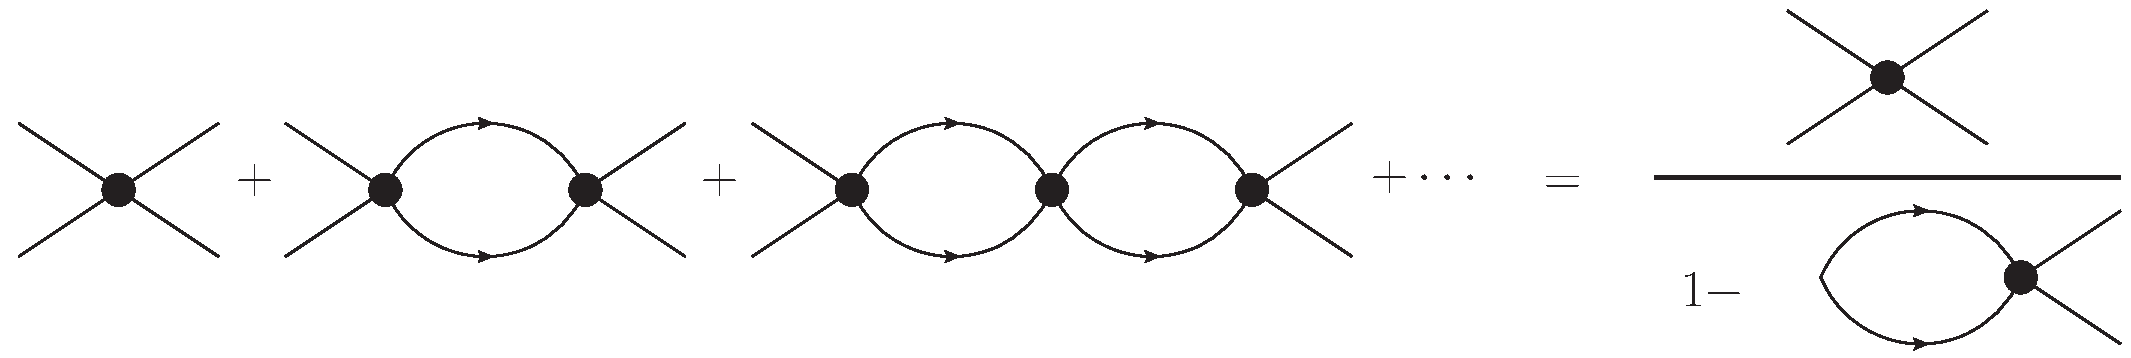
\includegraphics[width=\columnwidth]{figure/bubbleSum.pdf}
\caption{Bubble sum. Each line represents a propagator, each vertex represents $-i \sum_n C_{2n}(\Lambda) p^{2n}$, and the bubble is given by $I_0$ (see also \Figref{I0}).\label{fig:bubbleSum}}
\end{figure}

This bubble sum is a geometric series and gives, for the standard $T$-matrix, \cite{Kaplan:1998we,Beane:2003da}
\begin{equation}\label{eq:T matrix}
iT = \frac{-i\sum_n C_{2n}(\Lambda) p^{2n}}{1-I_0(p,\Lambda) \sum_n C_{2n}(\Lambda) p^{2n}},
\end{equation}
where $p$ is the relative momentum,  and $I_0(p,\Lambda)$ is a $D$-dependent function that arises from integrating the loop shown in \Figref{I0},
\begin{align}
    I_0(p)
    &=-i\int^{\Lambda}
        \frac { \mathrm {d}q_0}{2\pi}\ \frac{\mathrm { d } ^ { D } \vec{ q } } { (2\pi)^ { D } }
        \left( \frac { i } { \frac{E}{2} + q _ { 0 } - \frac{\vec{q}^2}{2m_1} + i \epsilon } \right)
        \left( \frac { i } { \frac{E}{2} - q _ { 0 } - \frac{\vec{q}^2}{2m_2} + i \epsilon } \right)
    \nonumber\\
    &=\frac{\Omega_D}{(2\pi)^D}\int^{\Lambda}  \mathrm { d } q \ q^{D-1}\left[\mathcal{P} \left( \frac { 1 } { E - \frac{\vec{q}^2}{2\mu} } \right)
-i\frac{\pi \mu}{q}\delta(q-\sqrt{2 \mu E})\right]
    \\
    &=\frac{\Omega_D}{(2\pi)^2}\frac{2\mu}{L^{D-2}}\int^{\Lambda L/2\pi}  \mathrm { d } n \ n^{D-1}\left[\mathcal{P} \left( \frac { 1 } { \left(\frac{pL}{2\pi}\right)^2 - n^2 } \right)
-i\frac{\pi^2}{L n}\delta\left(\frac{2\pi}{L}n -p\right)\right]
    \label{eq:I0}
\end{align}
where $\mathcal{P}$ refers to Principal (Cauchy) Value, we have used the on-shell condition $mE=p^2$, and the geometric factor
\begin{equation}
\Omega_D=\frac{2\pi^{D/2}}{\Gamma(D/2)}=
    \begin{cases}
        4\pi    &   (D=3)\\
        2\pi    &   (D=2)\\
        2       &   (D=1)
    \end{cases}\ ,
\end{equation}

\begin{figure}[h!]
    \center
    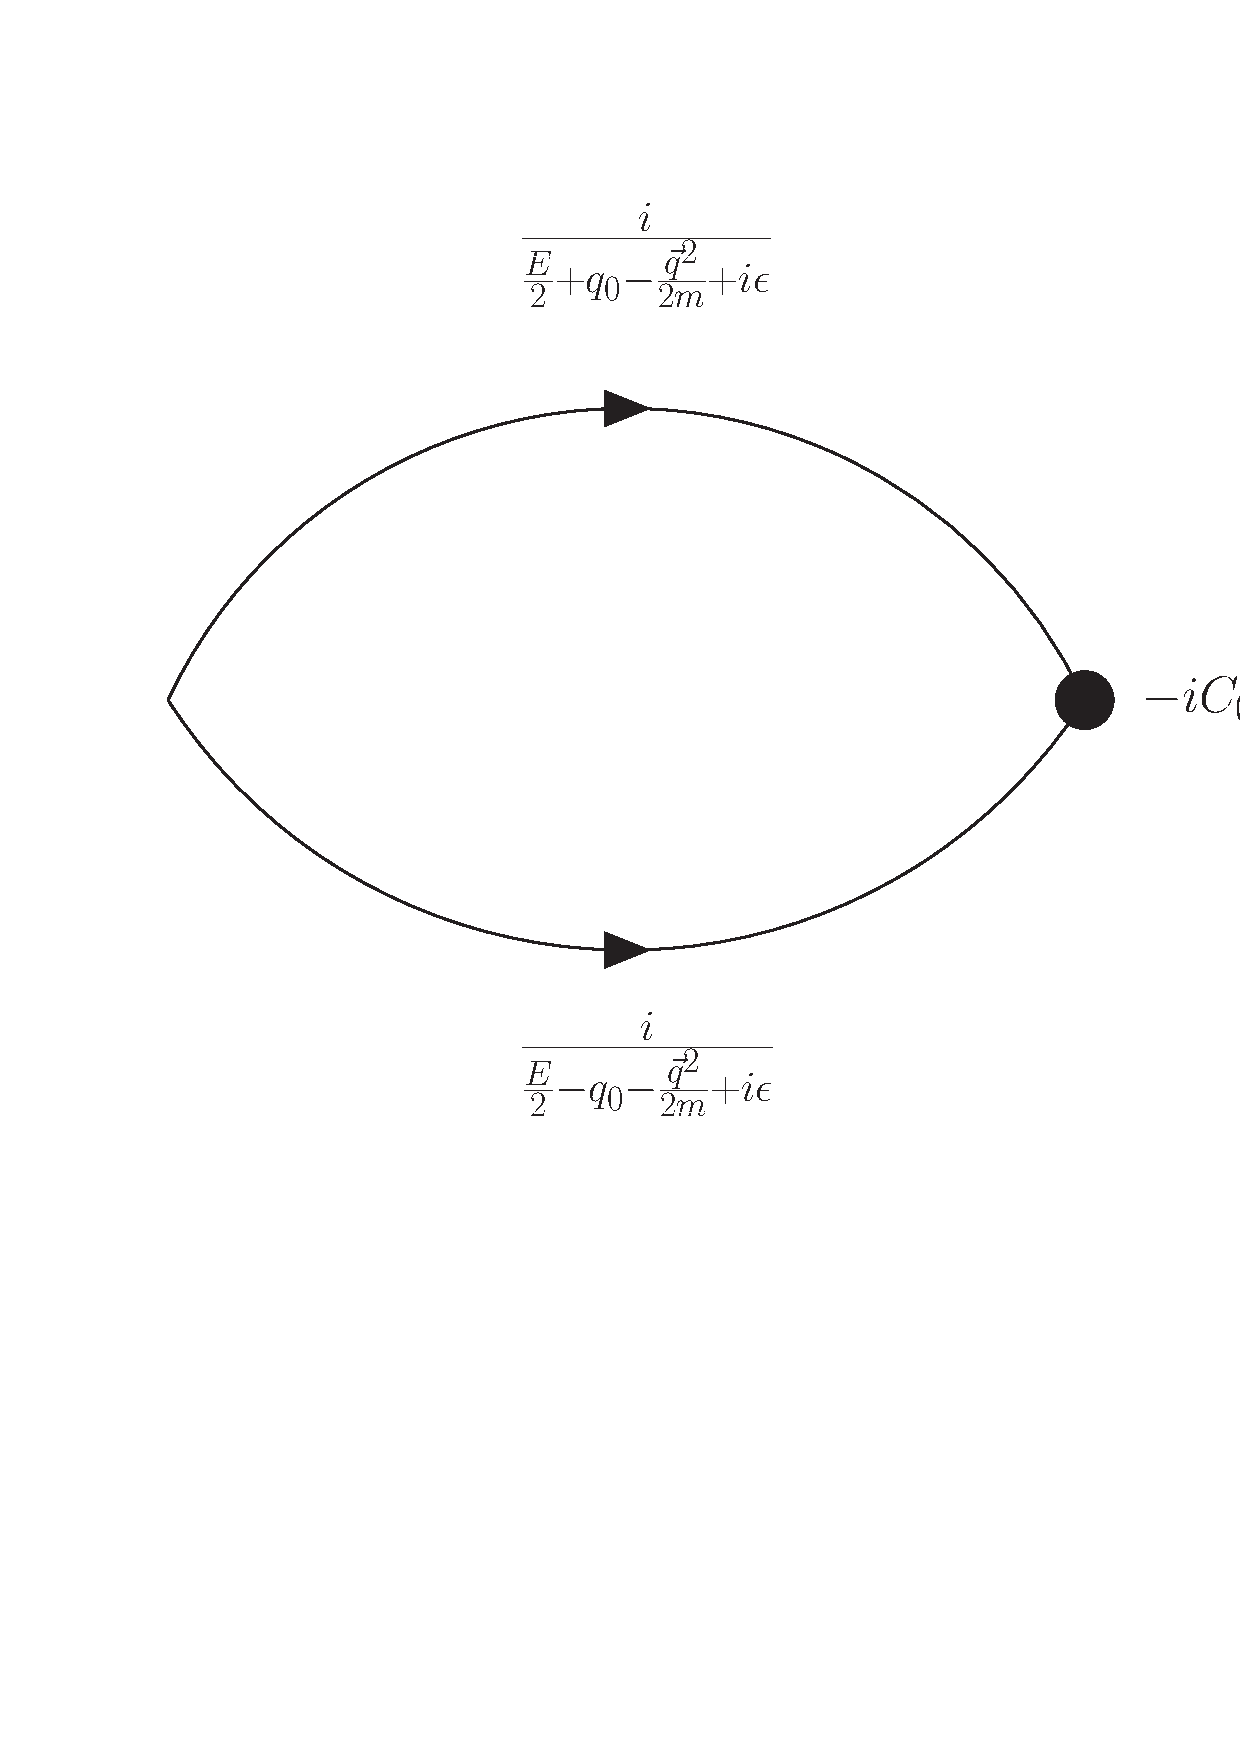
\includegraphics[width=.5\columnwidth]{figure/I0.pdf}
    \caption{
        Loop diagram contributing to the bubble sum.
        Because the potential is separable it factors out of the integral and $I_0$ is simply given by the loop of the two propagators.
    }
    \label{fig:I0}
\end{figure}

In the $s$-wave, the momentum-dependent $T$-matrix is related to the phase shift $\delta_0(p)$ by
\begin{equation}\label{eq:cot delta}
    i T = \frac{2}{\mu}\F_d\frac{i}{\cot \delta_0(p)-i}\ ,
\end{equation}
where
\begin{equation}
    \F_D
    =
    \begin{cases}
        \pi/p   & (D=3)\\
        1       & (D=2)\\
        p/2     & (D=1)
\end{cases}
\end{equation}
is a dimension-dependent kinematic factor.
This fixes the coefficients $C(\Lambda)$ as a function of the scattering data,
\begin{equation}\label{eq:IV pole}
    \frac{1}{\sum_n C_{2n}(\Lambda) p^{2n}}
    =
    I_0(p) - \frac{\mu}{2 \F_D}\left(\cot \delta_0(p) - i\right)
\end{equation}

In a finite volume, the energy eigenstates appear at poles of the $T$-matrix, so that
\begin{equation}\label{eq:FV pole}
    \frac{1}{\sum_n C_{2n}(\Lambda) p^{2n}} - I_{0,\FV}(p,L) = 0
\end{equation}
and the infinite-volume integral $I_0$ has been replaced by the matching finite-volume sum,
\begin{align}
I_{0,\FV}(p,L)
    &=-i\int \frac { \mathrm {d}q_0}{2\pi} \frac{1}{L^D}\sum_{\vec{q}}^{q < \Lambda} \left( \frac { i } { \frac{E}{2} + q _ { 0 } - \frac{\vec{q}^2}{2m_1} + i \epsilon } \right) \left( \frac { i } { \frac{E}{2} - q _ { 0 } - \frac{\vec{q}^2}{2m_2} + i \epsilon } \right)
    \\
    &=\frac{1}{L^D}\sum_{\vec{q}}^{q < \Lambda} \frac { 1 } { E - \frac{\vec{q}^2}{2\mu} }
    =\frac{2\mu}{(2\pi)^2 L^{D-2}} \sum_{\vec{n}}^{n < \frac{\Lambda L}{2\pi}} \frac{1}{x-n^2}
    &
    x &= \left( \frac{pL}{2\pi}\right)^2
\end{align}
where we have used the on-shell condition $2\mu E=p^2$.  Combining the infinite-volume and finite-volume relations \eqref{IV pole} and \eqref{FV pole} yields
\begin{equation}
    \frac{\mu}{2\F_D}(\cot\delta_0(p)-i) = I_0(p) - I_{0,\FV}(p),
\end{equation}
the finite-volume quantization condition.

Plugging our results for the integrals in, one finds
\begin{equation}
    \frac{1}{2\F_D}\left(\cot \delta_0(p) - i\right) = \frac{2}{(2\pi)^2 L^{D-2}}\left[ \left(\int_{\vec{n}} - \sum_{\vec{n}}\right) \frac{1}{x-n^2} + \frac{-i \pi^2\Omega_D}{L} \int \mathrm{d}n\ n^{D-2} \delta\left(\frac{2\pi}{L}n - p\right) \right]
\end{equation}
where both the sum and integral are cut off by a restriction on the magnitude of $n$, $n^2 < (\Lambda L / 2\pi)^2$, and the integral implicitly carries a factor of $\Omega_D n^{D-1}$.
In a seemingly miraculous (but required) cancellation, the imaginary part on the left hand side exactly cancels the last term in the sum on the right,\footnote{Actually, the cancellation is not \emph{so} miraculous---demanding it occur is essentially how $\F_D$ is determined.} and we are left with
\begin{equation}
    \cot \delta_0(p) = \frac{\F_D}{\pi^2 L^{D-2}} \left(\sum_{\vec{n}}-\int_{\vec{n}}\right) \frac{1}{n^2-x}
\end{equation}
where $x=(pL/2\pi)^2$ and we switched the sign of the sum and integral as well as the sign of the denominator.
Because we cut off the sum and the integral in exactly the same way, in dimensions where $I_0$ diverges with $\Lambda$, the divergence cancels against the divergence in the sum.
Let $N=\Lambda L/2\pi$.
Then, defining, with a finite cutoff on magnitude $N/2$,
\begin{equation}\label{eq:spherical cutoff S}
    S^{\spherical N}_D(x) = \left(\sum_{\vec{n}}- \int_{\vec{n}}\right) \frac{1}{x-n^2}
\end{equation}
where the $\spherical$ superscript reminds us that we cut off our sum and integral in a spherical way, based on the magnitude of $n<N/2$, we recover the usual \Luscher zeta functions by taking
\begin{equation}\label{eq:spherical S}
    S^\spherical_D(x)
    =
    \lim_{N\goesto\infty} S^{\spherical N}_D(x)
    =
    \lim_{N\rightarrow\infty}\left( \sum_{\vec{n}}^{n < N/2} \frac{1}{x-n^2} - \counterterm_D^\spherical \left(\frac{N}{2}\right)^{D-2}\right)
\end{equation}
where dimension-dependent counterterm $\counterterm_D^\spherical$ comes from the integral; we evaluate said counterterms in \Appref{counterterm/spherical}.
Finally,
\begin{equation}\label{eq:spherical quantization}
    \cot \delta_0(p) = \frac{\F_D}{\pi^2 L^{D-2}} S^\spherical_D(x).
\end{equation}
This is the usual \Luscher finite-volume quantization condition, and continuum-extrapolated energy levels should be fed through it to produce continuum-limit scattering data.
In three dimensions it is common to move the momentum dependence in $\F_D$ to the other size, as $p \cot\delta_0(p)$ is what appears in the effective range expansion, as we will discuss in \Secref{ere}.

\subsection{Numerical Results}

Now we can attempt a numerical characterization of fermions at unitarity.
Using the Hamiltonian \eqref{p space hamiltonian} in a three-dimensional cubic box of linear size $L$ with lattice spacing $\epsilon$, we tune the interaction strength $C(\epsilon)$ so that we always find the ground state to lie at the first zero of $S^{\spherical}_3$.
Once the strength is tuned to \todo{precision} we extract, using exact diagonalization, low-lying energy levels, holding the physical volume fixed.
In \Figref{unimproved spherical} we put those (finite-lattice-spacing) energy levels through \eqref{spherical quantization} to convert them to scattering data, and additionally perform a continuum extrapolation according to
\begin{equation}
    \text{\todo{Does the extrapolation depend on \nstep?}}
\end{equation}
with error bars given by \todo{something meaningful}.  \todo{Add continuum extrapolation as an appendix?  Collect data, provide a script?  Something!}

\begin{figure}[th]
    \includegraphics[width=\textwidth]{figure/db-contact-fv-c-fitted-parity-lg.pdf}
    \caption{We show the result of tuning the contact interaction so that the ground state matches the first zero of $S^{\spherical}_3$.  In the top row we show results for $L=1.0$~fm, in bottom we show $L=2.0$~fm, while in different columns we show different finite differences as described in \eqref{p space hamiltonian}, \eqref{gamma definition}, and \eqref{gamma determination}. \todo{WHAT DO THESE UNITS MEAN?  I would advocate just making things non-dimensional by using factors of $m$ or something?}}
    \label{fig:unimproved spherical}
\end{figure}

One can clearly see that without a continuum extrapolation, the finite-volume spectrum does not agree with the exactly-known flat solution that a contact interaction must provide.
That is, by foregoing a continuum extrapolation, we induce unphysical shape parameters.
In the remainder of this paper we improve this result markedly, so that the continuum limit towards unitarity is substantially easier.

\todo{Comment on the continuum-extrapolated results, which I can't do yet since they're not there :D}

In \Figref{finite a spherical} we show the result of tuning the contact interaction so that the ground state, when put through $S^{\spherical}_3$ yields a scattering length of \todo{something}.
Again, since the interaction is a contact interaction only, we expect a completely flat behavior.
In constrast, we see \todo{shapes that make us sad / curious}.

\begin{figure}[th]
    \includegraphics[width=\textwidth]{figure/db-contact-fv-c-fitted-parity-a-inv-lg.pdf}
    \caption{We results like \Figref{unimproved spherical}, but where the contact interaction was tuned so that the ground state matches yields $p\cot\delta = $\todo{some finite scattering length; part of \issue{19}} rather than to 0.  Similar deviation from completely flat behavior is apparent at any finite lattice spacing.}
    \label{fig:finite a spherical}
\end{figure}

\section{The Cartesian \Luscher Finite-Volume Counterterm}\label{sec:counterterm/cartesian}

The regulation of the sum in \eqref{cartesian S} is provided by
\begin{equation}
    \label{eq:cartesian S counterterm}
    \int_{-N/2}^{N/2} \mathrm{d}^Dn \frac{1}{n^2-x}
    =
    \left(\frac{N}{2}\right)^{D-2} \int_{-1}^{+1} \mathrm{d}^D\nu \frac{1}{\nu^2 - \xtilde}
\end{equation}
where we rescaled and $\xtilde=x/(N/2)$, and we can numerically evaluate the right-hand side with ease to achieve a complete improvement of the $S_D^{\cartesian N}$ function.

We can determine the counterterm in the three-dimensional Cartesian volume, evaluating the large-$N$ limit of the integral
\begin{equation}\label{eq:cartesian integral}
    \int_{-1}^{+1} \mathrm{d}^D\nu \frac{1}{\nu^2 - \xtilde}
\end{equation}
where $\nu^2 = \sum_d \nu_d^2$ summed on dimensions.
We can evaluate it as follows.  Consider the integral
\begin{equation}
	J^{\cartesian N}_0(\xtilde, m) = \int_{-1}^{+1} \mathrm{d}^D\nu \frac{e^{-m (\nu^2-\xtilde)}}{\nu^2-\xtilde}.
\end{equation}
Then, we know $\lim_{m\goesto\infty} J^{\cartesian N}_0(\xtilde, m) = 0$ and $J^{\cartesian N}_0(\xtilde, 0)$ is the integral in \eqref{cartesian integral} we wish to evaluate.
We can take advantage of the fundamental theorem of calculus,
\begin{align}
	\int_{-1}^{+1} \mathrm{d}^D\nu \frac{1}{\nu^2-\xtilde}
    &=
    J^{\cartesian N}_0(\xtilde,0) - J^{\cartesian N}_0(\xtilde,\infty)
		&&= 	\int_{\infty}^{0} dm\ \partial_m J^{\cartesian N}_0(\xtilde,m)
		% \\
		&&=	\int_{\infty}^{0} dm\ \int_{-1}^{+1} \mathrm{d}^D\nu -e^{-m (\nu^2-\xtilde)}
		\nonumber\\
		&&&=	\int_0^\infty dm\ e^{m \xtilde^2}\left(\int_{-1}^{+1} d\nu\ e^{-m \nu^2}\right)^D
		% \\
		&&=	\int_0^\infty dm\ e^{m\xtilde}\left(\sqrt{\frac{\pi}{m}} \erf(\sqrt{m})\right)^D
        \nonumber\\
    &&&=
    \pi^{D/2} \int_{0}^{\infty} 2\mu\; \mathrm{d}\mu\; e^{\xtilde \mu^2} \left(\frac{\erf(\mu)}{\mu}\right)^D
\end{align}
where we exchange the order of partial differentiation by $m$ and momenta integration, recognize the resulting integral as three identical copies of the same integral (as long as the volume is a cube), and evaluate it, yielding the error function, and finally change variables $m\goesto\mu^2$, easing the numerical integration.
When $\xtilde\leq0$ our procedure is legitimate, and for $\xtilde=0$ in three dimensions one finds $2.75634$ so that
\begin{equation}
    \label{eq:cartesian counterterm}
    \counterterm^\cartesian_3 \left(\frac{N}{2}\right) = \lim_{N\goesto\infty}\int_{-N/2}^{+N/2} \mathrm{d}^3n \frac{1}{n^2} = 15.34824844488746404710\ \left(\frac{N}{2}\right)
\end{equation}
and more digits are readily available; this constant appears in \eqref{cartesian S}.
This can be compared to the spherical counterterm, which we can read off from \eqref{improved spherical S}, where the counter term can be seen to be $4\pi \approx 12.6 $; that the Cartesian result is larger reflects the fact that more of the momentum space is included in the integration domain for a fixed $N$, as discussed in \Secref{cartesian}.

For $D\geq3$ spatial dimensions one can immediately use the same method to find the leading divergences.
For four dimensions one finds $17.14741624920737 (N/2)^2$, $24.49922817921121 (N/2)^3$ for five dimensions, for six dimensions $38.50096808074375 (N/2)^4$, and so on.  However, in these higher dimensions we must also subtract subleading divergences, which requires the determination of additional counterterms we do not here compute.

The logarithmic divergence in two dimensions must be handled especially carefully.
\todo{TOM'S MAGIC INTEGRAL AND CATALAN'S CONSTANT}.

In fact, we can execute a similar construction in three (and higher) dimensions.  In three dimensions, \todo{TOM'S G+POLYLOG MAGIC}.

\section{Matching, and the Effective Range Expansion}\label{sec:ere}

We can use the effective range expansion to express the scattering data as the sum of some known terms that do not vanish at low momentum and a series in $p^2$.  The expansion differs in different dimensions,
\begin{align}
    p\ (\cot \delta_0(p) - i)
    &=
    -\frac{1}{a} - ip + \frac{1}{2} r_0 p^2 \sum_j s_j (r_0^2 p^2)^j
    &
    (D&=3)
    \nonumber\\
    \cot \delta_0(p) - i
    &=
    \frac{2}{\pi} \log(a p) -i + \frac{1}{2} r_0^2 p^2 \sum_j s_j (r_0^2 p^2)^j
    &
    (D&=2)
    \\\nonumber
    \frac{\cot\delta_0(p)-i}{p}
    &=
    -\frac{i}{p} + a + \frac{1}{2} r_0^3 p^2 \sum_j s_j( r_0^2 p^2)^j
    &
    (D&=1)
\end{align}
where $a$ is the scattering length, $r_0$ the length scale called the effective range, and the $s_j$ are dimensionless shape parameters.
We can solve for the phase shift and encapsulate the low-energy pieces of the right-hand side into
\begin{equation}
    \lowEnergyA(p) =
    \begin{cases}
        -\frac{1}{ap}           &   (D=3)\\
        \frac{2}{\pi} \log ap   &   (D=2)\\
        ap                      &   (D=1)
    \end{cases}\ ,
\end{equation}
so that
\begin{equation}\label{eq:ERE}
    \cot \delta_0(p) - i = -i + \lowEnergyA(p) + \frac{1}{2} (r_0 p)^{4-D} \sum_j s_j \left(r_0^2p^2\right)^j.
\end{equation}
We can take this expression and plug it into \eqref{IV pole}, matching the dependence on $p$.
Using the spherical $I_0(p)$, one finds
\begin{align}
    \nonumber
    D&=3:
    &
    0&=\frac{4 \pi}{m C_0}-\frac{1}{a} + \frac{2N}{L}
    &
    0&=- \frac{4 \pi C_2}{m C_0^2} + \frac{1}{2}r_0 s_0 - \frac{2 L}{N \pi^2}
    &
    0&=\frac{4\pi(C_2^2-C_0 C_4)}{m C_0^3} + \frac{1}{2} r_0^3 s_1 - \frac{2L^3}{3\pi^4 N^3}
    &\ldots&
    \\
    D&=2:
    &
    0&=\frac{4}{m C_0} + \frac{2}{\pi} \log \frac{a N \pi}{L}
    &
    0&=- \frac{4 C_2}{m C_0^2} + \frac{1}{2}r_0^2 s_0  - \frac{L^2}{N^2 \pi^3}
    &
    0&=\frac{4(C_2^2-C_0 C_4)}{m C_0^3} + \frac{1}{2} r_0^4 s_1 - \frac{2 L^4}{4\pi^5 N^4}
    &\ldots&
    \\
    D&=1:
    &
    0&=\frac{2}{m C_0}+a-\frac{2L}{\pi^2N}
    &
    0&=- \frac{2 C_2}{m C_0^2} + \frac{1}{2}r_0^3 s_0 - \frac{2 L^3}{3N^3 \pi^4}
    &
    0&=\frac{2(C_2^2-C_0 C_4)}{m C_0^3} + \frac{1}{2} r_0^5 s_1 - \frac{2 L^5}{5\pi^6 N^5 }
    &\ldots&
    \nonumber
\end{align}
where $N/2$ is the cutoff on the integral, the first term in each relation comes from expanding $1/\sum_n C_{2n} p^{2n}$, the second from the effective range expansion \eqref{ERE}, and the third from expanding $I_0$ as a function of $p$, holding a fixed cutoff.  These equations can be solved order-by-order for the coefficients in the potential, or, if we know the coefficients, we can read these equations as determining the scattering data ($r_0$ and $s_j$) and how to correct for a finite cutoff.
\todo{Using $L=N\epsilon$ and $\epsilon=\pi/\Lambda$ I have checked that setting $C_{>0}=0$ reproduces 3-2-1-blastoff's (16), (17), (18) for D=3, (25) for D=2, and, when the cutoff is infinite, (28) for D=1.}

Of special note is the matching condition for $C_0$ when $D=2$, where the momentum dependence at small $p$ is logarithmic, and we cannot take an independent continuum and finite-volume limit.
\todo{What are we supposed again?  I used to understand this.  There's some dimensional transmutation magic going on here.}

We can also use this understanding to construct an improved \Luscher's formula.
Note that when passing from the cut off \eqref{spherical cutoff S} to \eqref{spherical S} we replaced the integral with its limiting value, the divergence-cancelling counterterm.
Rather than jump straight to the leading dependence on the cutoff, we can subtract subleading terms as well.
One finds, truncating our improvement scheme at order $J$,
\begin{align}
    S_3^\spherical(x)  = \lim_{N\goesto\infty} S^{\spherical N}_3(x)
    &=
    \lim_{N\goesto\infty}\left[\sum_{\vec{n}}^{n<N/2} \frac{1}{x-n^2}
        + 4\pi \sum_{j=0}^{J} \frac{x^j}{2j-1} \left(\frac{N}{2}\right)^{-(2j-1)}
    \right]
    &
    (D&=3)
    \\
    S_2^\spherical(x)  = \lim_{N\goesto\infty} S^{\spherical N}_2(x)
    &=
    \lim_{N\goesto\infty}\left[\sum_{\vec{n}}^{n<N/2} \frac{1}{x-n^2}
        + \pi \log \frac{x}{(N/2)^2}
        + \pi \sum_{j=1}^{J} \frac{x^j}{j} \left(\frac{N}{2}\right)^{-2j}
    \right]
    &
    (D&=2)
    \\
    S_1^\spherical(x)  = \lim_{N\goesto\infty} S^{\spherical N}_1(x)
    &=
    \lim_{N\goesto\infty}\left[\sum_{\vec{n}}^{n<N/2} \frac{1}{x-n^2}
        + 2 \sum_{j=0}^{J} \frac{x^j}{2j+1}\left(\frac{N}{2}\right)^{-(2j+1)}
        \right]
    &
    (D&=1)
\end{align}


\begin{center}
    \boxed{\textrm{{\color{red}REALLY TOUGH CHALLENGE: TELL THE ABOVE STORY WITH A CARTESIAN CUTOFF?}}}
\end{center}

\todo{I'm no longer convinced that (assuming you take the cutoff to infinity) spherical and cartesian should be different.  I think they should come out the same.}

\section{The Dispersion \Luscher Finite-Volume Counterterm}\label{sec:counterterm/dispersion}

To evaluate the infinite-volume integral in \eqref{dispersion S},
\begin{equation}
    \left(\frac{N}{2}\right)^{D-2}
    4\pi^2 \int_{-N/2}^{+N/2} \mathrm{d}^Dn\; \PV \frac{1}{N^2 \sum_{ds} \gamma^{(\nstep)}_s \cos \frac{2\pi n_d s}{N} - x}
    =
    4\pi^2 \left(\frac{N}{2}\right) \int_{-1}^{+1} \mathrm{d}^D\nu\; \PV \frac{1}{4\sum_{ds} \gamma^{(\nstep)}_s \cos \pi \nu s - \tilde{x}}
\end{equation}
where as in the Cartesian case we rescaled and $\tilde{x} = x/(N/2)^2$.
Note that when we replace the sum over dimensions and steps with the exact $p^2$ result $(\pi \nu)^2$ and let $\tilde{x}$ vanish, we can match \eqref{cartesian S counterterm}.

We can use the same trick to isolate the leading behavior in $N/2$, introducing the dispersion relation in the exponent rather than $n^2$.
One finds a coefficient multiplying $(N/2)^{D-2}$,
\begin{equation}
    \label{eq:dispersion counterterm}
    \mathcal{L}^{\dispersion (\nstep)}_D = 4 \pi^2 \int_{0}^{\infty} 2\mu\; \mathrm{d}\mu\; \left(\int_{-1}^{+1} \mathrm{d}\nu\; e^{-4\mu^2 \sum_s \gamma_s^{(\nstep)} \cos \pi \nu s}\right)^D
\end{equation}
which can be numerically evaluated quickly, assuming one has the dispersion relation coefficients in hand.
In \Figref{nstep counterterm} we show this counterterm and how it differs from the $\nstep=\infty$ counterterm.

\begin{figure}
    \includegraphics{figure/counterterm-nstep.pdf}
    \caption{In the top panel we show the dispersion counterterm $\mathcal{L}^{\dispersion (\nstep)}_{3}$in \eqref{dispersion counterterm} as a function of $\nstep$, and the $\nstep=\infty$ result, which is the same as the Cartesian result $\mathcal{L}^{\cartesian}_3$, as a dashed line.  In the bottom panel we show a better view into how the counterterm converges to the Cartesian one.
    }
    \label{fig:nstep counterterm}
\end{figure}

\section{Conclusion}\label{sec:conclusion}

We presented a tuning prescription for a two-particle lattice system interacting through a contact interaction in 1-, 2- and 3-dimensions.
For this interaction, the tuning prescription allows us to compute infinite volume continuum scattering observables %(which are independent from unphysical artifacts)
from data computed in the finite volume and discrete space.
Furthermore we derived a \Luscher-like formalism which directly converts the associated finite-volume finite-spacing spectra to infinite-volume continuum phase shifts for the contact interaction.

In 3-dimensions, we analyzed three different approaches in detail:
\begin{enumerate}
	\item we tuned the interaction parameter in a finite volume with a finite lattice spacing to the intersections of the \Luscher zeta function and the phase shifts, extracted the continuum-extrapolated spectrum, and used the same \Luscher zeta function to re-obtain the phase shifts,
	\item we repeated the same procedure without extrapolating the spectrum to the continuum and found phase shifts with induced energy-dependence,
	\item we derived a dispersion-aware zeta function which removed the energy dependence in the phase shifts,
	\item we perturbatively computed the discretization dependent coefficients which describe the difference in the effective range expansion between continuum extrapolated results and results obtained at a finite spacing.
\end{enumerate}

The first approach follows the logic of \Luscher's original work and reproduces the expected phase shifts.
Even though we had full control over numerical errors, the continuum extrapolation of the spectrum suffered from systematic artifacts and induced significant uncertainties (on a relative scale) when put through the zeta function.
In general the best discretization allows the best extrapolation and for smaller energy values, continuum results are more precise.
It is possible to find discretizations in which the finite spacing spectrum is close to its continuum result but the extrapolation uncertainties can be larger because of non-monotonic behavior of individual energy levels in dependence of the lattice spacing.

The second approach, applying the infinite-volume map to finite-spacing energy levels---the approach of most recent lattice QCD work---suffers from notable discretization artifacts.
These artifacts induce an energy dependence in the phase shifts at any finite spacing.
For example, we found induced effective range (and higher order) effects which we analytically estimated.
These induced terms can be extrapolated to zero in a stable manner in the continuum if one only considers energy values in the scaling region.
We provide tables of coefficients which estimate the size of errors in the phase shifts caused by the discretization.

The third approach allows a direct conversion from finite-spacing finite-volume energy levels to continuum infinite-volume phase shifts without any extrapolation.
Thus it was possible to consistently tune the interaction parameter to high precision.
Further, this tuning allows one to distinguish between kinetic discretization effects and discretization effects affecting the regulator of the theory and thus allows one to determine the interaction consistently.

Finally, we repeated our three-dimensional analysis above to both one- and two-dimensional systems.
The latter is further complicated by logarithmic singularities as opposed to power law divergences, and so here we proposed a slightly modified \Luscher equation in two dimensions to account for the logarithmic singularity near $p\sim 0$.
In both cases our results are consistent with those found in the literature.

We expect our discretization-specific tuning for the contact interaction parameter can be carried beyond the two-body sector and used in many-body computations, so that calculations of the Bertsch parameter should benefit from having a systematically correct tuned interaction, which we plan to investigate in future work.
We note, however, that while it would be desirable to find a similar dispersion formalism and tuning prescription for any interaction (for example, finite-range interactions), the derivation of this prescription in this case would depend on an explicit knowledge of the short-distance parts of the interaction.
We do not rule out, however, that our dispersion formalism might be applicable to other specific interactions, or maybe even generalizes in a perturbative manner for general interactions.  %, it seems unlikely to us that it generalizes to scenarios where the effective interaction between emergent objects is not explicitly known.

%I like coffee a lot.
%Without coffee, I would be tired each morning.
%Accounting for the tiredness overhead, I am certain that my productivity would be considerably smaller.
%Thus I think there should be free coffee for any scientist.
%Well, for any human (which is capable of properly digesting coffee) I guess.
%Cheers to coffee!


\appendix
\section{Misc}

We can put the derivation of the counter terms etc. in appendices.

Do we want to put tables?  Make numerical data directly available?  We should be good, reproducible scientists.

\section{The Usual, Spherical \Luscher's Formula}\label{sec:spherical}


Here we present a $D$-dimensional derivation of \Luscher's formula that roughly follows \Ref{Beane:2003da}, although the technology and sophistication of the finite-volume formalism has grown substantially \todo{cite cite cite}.  Assuming an interaction given by an tower of derivative contact operators
\begin{equation}
    V(p) = +\sum_n C_{2n}(\Lambda) p^{2n}
\end{equation}
where the interaction strengths depend on the regulator and carry spatial-dimension-dependent units.
The scattering amplitude is given by the bubble sum depicted in \Figref{bubbleSum}.

\begin{figure}[ht!]
\center
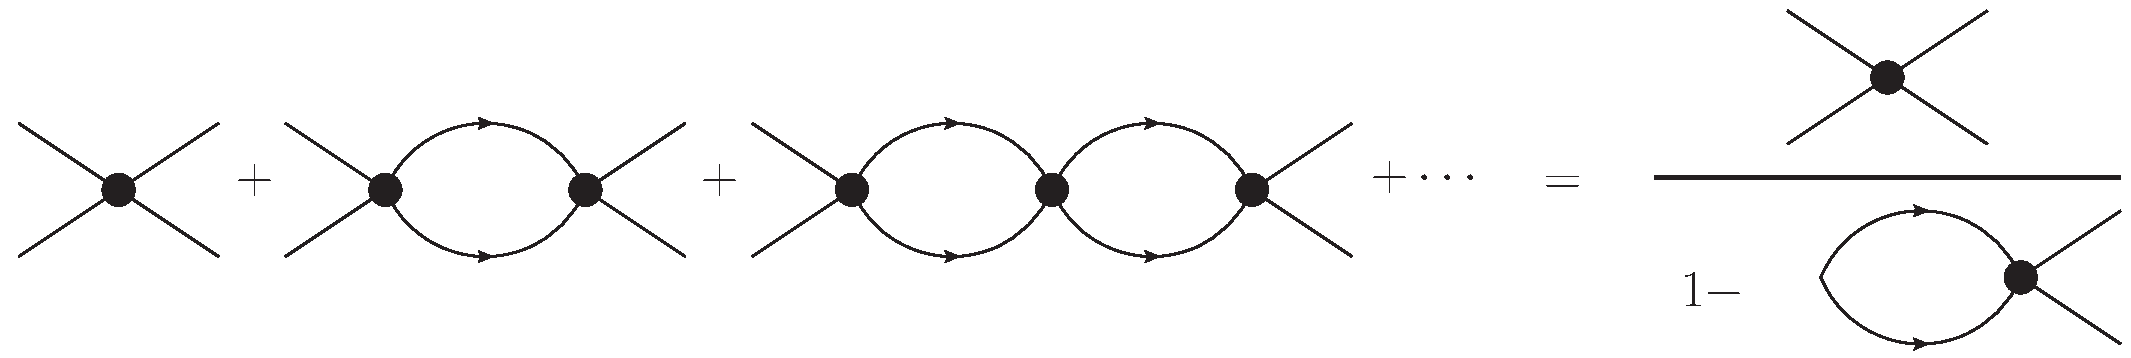
\includegraphics[width=\columnwidth]{figure/bubbleSum.pdf}
\caption{Bubble sum. Each line represents a propagator, each vertex represents $-i \sum_n C_{2n}(\Lambda) p^{2n}$, and the bubble is given by $I_0$ (see also \Figref{I0}).\label{fig:bubbleSum}}
\end{figure}

This bubble sum is a geometric series and gives, for the standard $T$-matrix, \cite{Kaplan:1998we,Beane:2003da}
\begin{equation}\label{eq:T matrix}
iT = \frac{-i\sum_n C_{2n}(\Lambda) p^{2n}}{1-I_0(p,\Lambda) \sum_n C_{2n}(\Lambda) p^{2n}},
\end{equation}
where $p$ is the relative momentum,  and $I_0(p,\Lambda)$ is a $D$-dependent function that arises from integrating the loop shown in \Figref{I0},
\begin{align}
    I_0(p)
    &=-i\int^{\Lambda}
        \frac { \mathrm {d}q_0}{2\pi}\ \frac{\mathrm { d } ^ { D } \vec{ q } } { (2\pi)^ { D } }
        \left( \frac { i } { \frac{E}{2} + q _ { 0 } - \frac{\vec{q}^2}{2m_1} + i \epsilon } \right)
        \left( \frac { i } { \frac{E}{2} - q _ { 0 } - \frac{\vec{q}^2}{2m_2} + i \epsilon } \right)
    \nonumber\\
    &=\frac{\Omega_D}{(2\pi)^D}\int^{\Lambda}  \mathrm { d } q \ q^{D-1}\left[\mathcal{P} \left( \frac { 1 } { E - \frac{\vec{q}^2}{2\mu} } \right)
-i\frac{\pi \mu}{q}\delta(q-\sqrt{2 \mu E})\right]
    \\
    &=\frac{\Omega_D}{(2\pi)^2}\frac{2\mu}{L^{D-2}}\int^{\Lambda L/2\pi}  \mathrm { d } n \ n^{D-1}\left[\mathcal{P} \left( \frac { 1 } { \left(\frac{pL}{2\pi}\right)^2 - n^2 } \right)
-i\frac{\pi^2}{L n}\delta\left(\frac{2\pi}{L}n -p\right)\right]
    \label{eq:I0}
\end{align}
where $\mathcal{P}$ refers to Principal (Cauchy) Value, we have used the on-shell condition $mE=p^2$, and the geometric factor
\begin{equation}
\Omega_D=\frac{2\pi^{D/2}}{\Gamma(D/2)}=
    \begin{cases}
        4\pi    &   (D=3)\\
        2\pi    &   (D=2)\\
        2       &   (D=1)
    \end{cases}\ ,
\end{equation}

\begin{figure}[h!]
    \center
    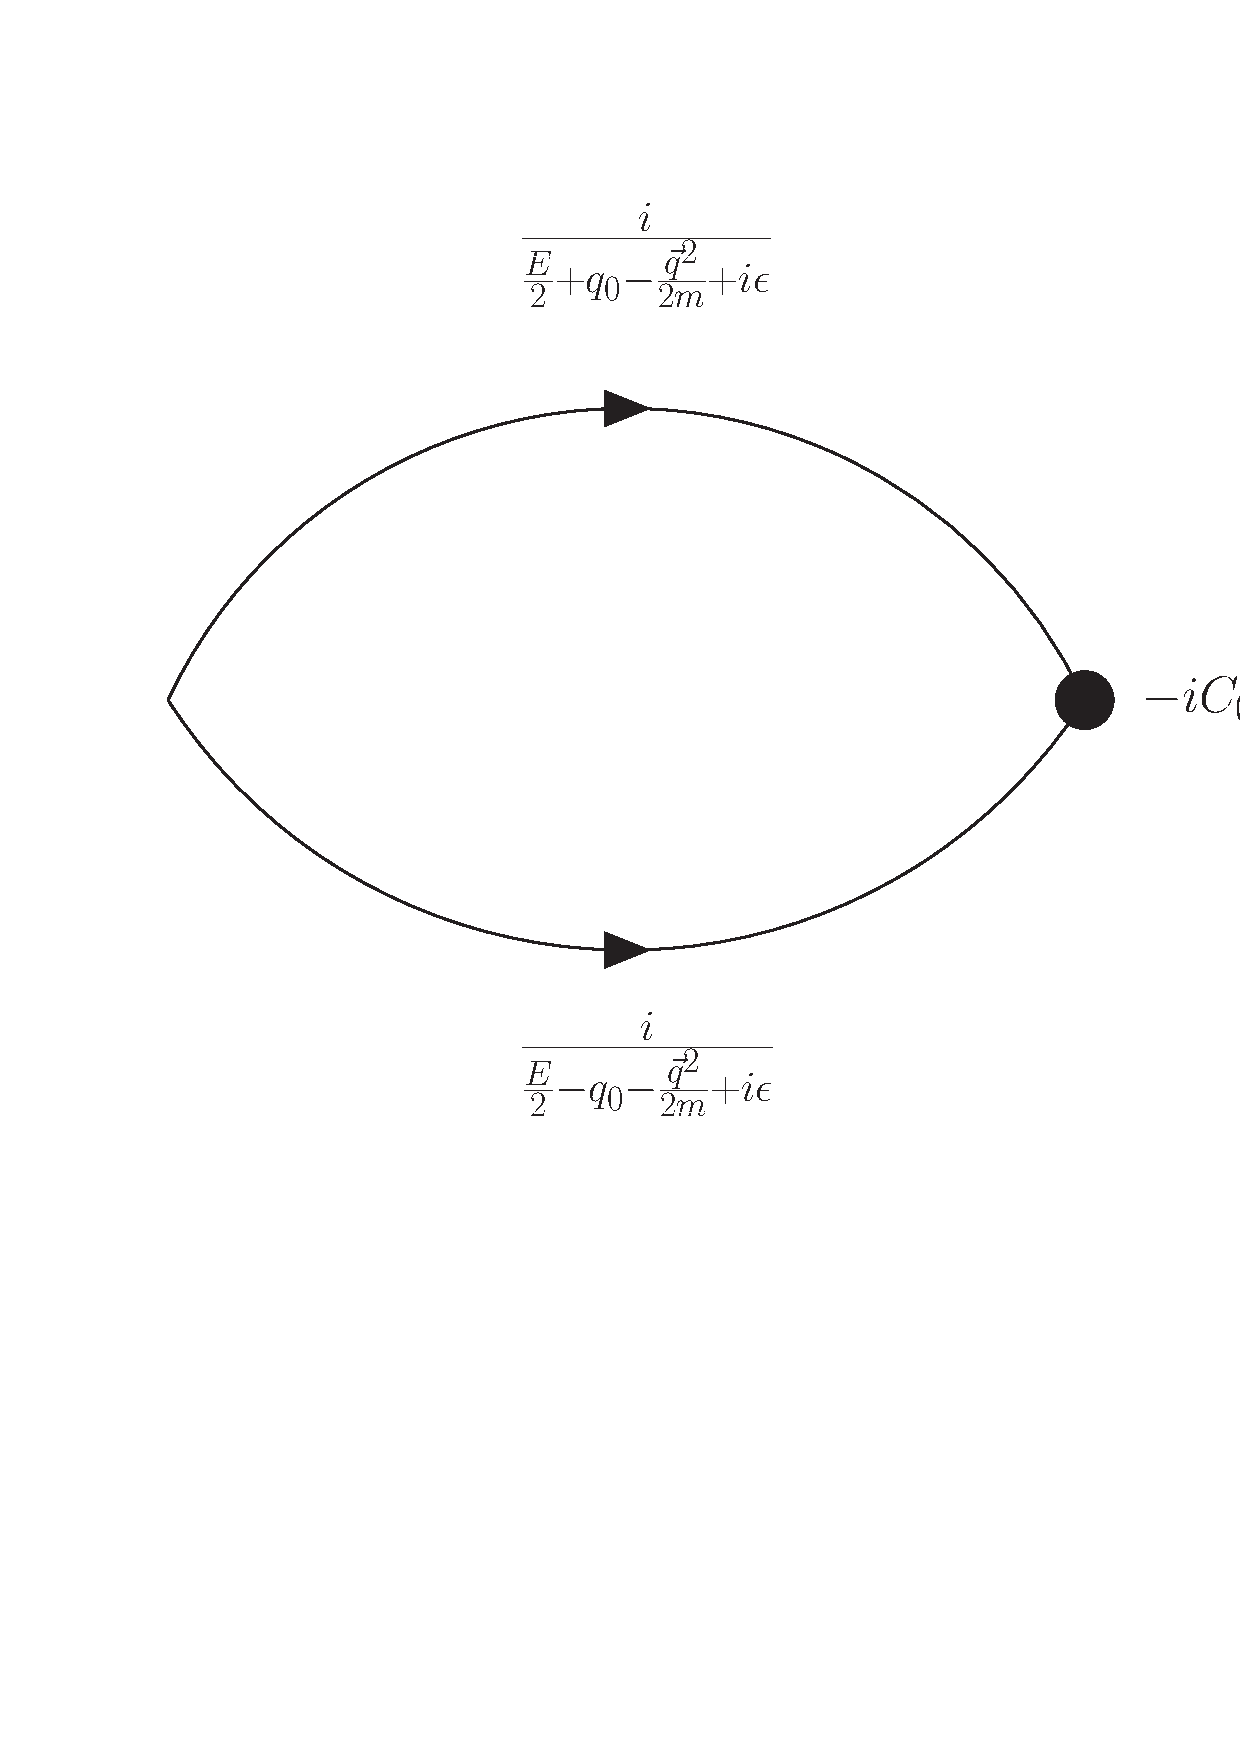
\includegraphics[width=.5\columnwidth]{figure/I0.pdf}
    \caption{
        Loop diagram contributing to the bubble sum.
        Because the potential is separable it factors out of the integral and $I_0$ is simply given by the loop of the two propagators.
    }
    \label{fig:I0}
\end{figure}

In the $s$-wave, the momentum-dependent $T$-matrix is related to the phase shift $\delta_0(p)$ by
\begin{equation}\label{eq:cot delta}
    i T = \frac{2}{\mu}\F_d\frac{i}{\cot \delta_0(p)-i}\ ,
\end{equation}
where
\begin{equation}
    \F_D
    =
    \begin{cases}
        \pi/p   & (D=3)\\
        1       & (D=2)\\
        p/2     & (D=1)
\end{cases}
\end{equation}
is a dimension-dependent kinematic factor.
This fixes the coefficients $C(\Lambda)$ as a function of the scattering data,
\begin{equation}\label{eq:IV pole}
    \frac{1}{\sum_n C_{2n}(\Lambda) p^{2n}}
    =
    I_0(p) - \frac{\mu}{2 \F_D}\left(\cot \delta_0(p) - i\right)
\end{equation}

In a finite volume, the energy eigenstates appear at poles of the $T$-matrix, so that
\begin{equation}\label{eq:FV pole}
    \frac{1}{\sum_n C_{2n}(\Lambda) p^{2n}} - I_{0,\FV}(p,L) = 0
\end{equation}
and the infinite-volume integral $I_0$ has been replaced by the matching finite-volume sum,
\begin{align}
I_{0,\FV}(p,L)
    &=-i\int \frac { \mathrm {d}q_0}{2\pi} \frac{1}{L^D}\sum_{\vec{q}}^{q < \Lambda} \left( \frac { i } { \frac{E}{2} + q _ { 0 } - \frac{\vec{q}^2}{2m_1} + i \epsilon } \right) \left( \frac { i } { \frac{E}{2} - q _ { 0 } - \frac{\vec{q}^2}{2m_2} + i \epsilon } \right)
    \\
    &=\frac{1}{L^D}\sum_{\vec{q}}^{q < \Lambda} \frac { 1 } { E - \frac{\vec{q}^2}{2\mu} }
    =\frac{2\mu}{(2\pi)^2 L^{D-2}} \sum_{\vec{n}}^{n < \frac{\Lambda L}{2\pi}} \frac{1}{x-n^2}
    &
    x &= \left( \frac{pL}{2\pi}\right)^2
\end{align}
where we have used the on-shell condition $2\mu E=p^2$.  Combining the infinite-volume and finite-volume relations \eqref{IV pole} and \eqref{FV pole} yields
\begin{equation}
    \frac{\mu}{2\F_D}(\cot\delta_0(p)-i) = I_0(p) - I_{0,\FV}(p),
\end{equation}
the finite-volume quantization condition.

Plugging our results for the integrals in, one finds
\begin{equation}
    \frac{1}{2\F_D}\left(\cot \delta_0(p) - i\right) = \frac{2}{(2\pi)^2 L^{D-2}}\left[ \left(\int_{\vec{n}} - \sum_{\vec{n}}\right) \frac{1}{x-n^2} + \frac{-i \pi^2\Omega_D}{L} \int \mathrm{d}n\ n^{D-2} \delta\left(\frac{2\pi}{L}n - p\right) \right]
\end{equation}
where both the sum and integral are cut off by a restriction on the magnitude of $n$, $n^2 < (\Lambda L / 2\pi)^2$, and the integral implicitly carries a factor of $\Omega_D n^{D-1}$.
In a seemingly miraculous (but required) cancellation, the imaginary part on the left hand side exactly cancels the last term in the sum on the right,\footnote{Actually, the cancellation is not \emph{so} miraculous---demanding it occur is essentially how $\F_D$ is determined.} and we are left with
\begin{equation}
    \cot \delta_0(p) = \frac{\F_D}{\pi^2 L^{D-2}} \left(\sum_{\vec{n}}-\int_{\vec{n}}\right) \frac{1}{n^2-x}
\end{equation}
where $x=(pL/2\pi)^2$ and we switched the sign of the sum and integral as well as the sign of the denominator.
Because we cut off the sum and the integral in exactly the same way, in dimensions where $I_0$ diverges with $\Lambda$, the divergence cancels against the divergence in the sum.
Let $N=\Lambda L/2\pi$.
Then, defining, with a finite cutoff on magnitude $N/2$,
\begin{equation}\label{eq:spherical cutoff S}
    S^{\spherical N}_D(x) = \left(\sum_{\vec{n}}- \int_{\vec{n}}\right) \frac{1}{x-n^2}
\end{equation}
where the $\spherical$ superscript reminds us that we cut off our sum and integral in a spherical way, based on the magnitude of $n<N/2$, we recover the usual \Luscher zeta functions by taking
\begin{equation}\label{eq:spherical S}
    S^\spherical_D(x)
    =
    \lim_{N\goesto\infty} S^{\spherical N}_D(x)
    =
    \lim_{N\rightarrow\infty}\left( \sum_{\vec{n}}^{n < N/2} \frac{1}{x-n^2} - \counterterm_D^\spherical \left(\frac{N}{2}\right)^{D-2}\right)
\end{equation}
where dimension-dependent counterterm $\counterterm_D^\spherical$ comes from the integral; we evaluate said counterterms in \Appref{counterterm/spherical}.
Finally,
\begin{equation}\label{eq:spherical quantization}
    \cot \delta_0(p) = \frac{\F_D}{\pi^2 L^{D-2}} S^\spherical_D(x).
\end{equation}
This is the usual \Luscher finite-volume quantization condition, and continuum-extrapolated energy levels should be fed through it to produce continuum-limit scattering data.
In three dimensions it is common to move the momentum dependence in $\F_D$ to the other size, as $p \cot\delta_0(p)$ is what appears in the effective range expansion, as we will discuss in \Secref{ere}.

\subsection{Numerical Results}

Now we can attempt a numerical characterization of fermions at unitarity.
Using the Hamiltonian \eqref{p space hamiltonian} in a three-dimensional cubic box of linear size $L$ with lattice spacing $\epsilon$, we tune the interaction strength $C(\epsilon)$ so that we always find the ground state to lie at the first zero of $S^{\spherical}_3$.
Once the strength is tuned to \todo{precision} we extract, using exact diagonalization, low-lying energy levels, holding the physical volume fixed.
In \Figref{unimproved spherical} we put those (finite-lattice-spacing) energy levels through \eqref{spherical quantization} to convert them to scattering data, and additionally perform a continuum extrapolation according to
\begin{equation}
    \text{\todo{Does the extrapolation depend on \nstep?}}
\end{equation}
with error bars given by \todo{something meaningful}.  \todo{Add continuum extrapolation as an appendix?  Collect data, provide a script?  Something!}

\begin{figure}[th]
    \includegraphics[width=\textwidth]{figure/db-contact-fv-c-fitted-parity-lg.pdf}
    \caption{We show the result of tuning the contact interaction so that the ground state matches the first zero of $S^{\spherical}_3$.  In the top row we show results for $L=1.0$~fm, in bottom we show $L=2.0$~fm, while in different columns we show different finite differences as described in \eqref{p space hamiltonian}, \eqref{gamma definition}, and \eqref{gamma determination}. \todo{WHAT DO THESE UNITS MEAN?  I would advocate just making things non-dimensional by using factors of $m$ or something?}}
    \label{fig:unimproved spherical}
\end{figure}

One can clearly see that without a continuum extrapolation, the finite-volume spectrum does not agree with the exactly-known flat solution that a contact interaction must provide.
That is, by foregoing a continuum extrapolation, we induce unphysical shape parameters.
In the remainder of this paper we improve this result markedly, so that the continuum limit towards unitarity is substantially easier.

\todo{Comment on the continuum-extrapolated results, which I can't do yet since they're not there :D}

In \Figref{finite a spherical} we show the result of tuning the contact interaction so that the ground state, when put through $S^{\spherical}_3$ yields a scattering length of \todo{something}.
Again, since the interaction is a contact interaction only, we expect a completely flat behavior.
In constrast, we see \todo{shapes that make us sad / curious}.

\begin{figure}[th]
    \includegraphics[width=\textwidth]{figure/db-contact-fv-c-fitted-parity-a-inv-lg.pdf}
    \caption{We results like \Figref{unimproved spherical}, but where the contact interaction was tuned so that the ground state matches yields $p\cot\delta = $\todo{some finite scattering length; part of \issue{19}} rather than to 0.  Similar deviation from completely flat behavior is apparent at any finite lattice spacing.}
    \label{fig:finite a spherical}
\end{figure}

\section{The Cartesian \Luscher Finite-Volume Counterterm}\label{sec:counterterm/cartesian}

The regulation of the sum in \eqref{cartesian S} is provided by
\begin{equation}
    \label{eq:cartesian S counterterm}
    \int_{-N/2}^{N/2} \mathrm{d}^Dn \frac{1}{n^2-x}
    =
    \left(\frac{N}{2}\right)^{D-2} \int_{-1}^{+1} \mathrm{d}^D\nu \frac{1}{\nu^2 - \xtilde}
\end{equation}
where we rescaled and $\xtilde=x/(N/2)$, and we can numerically evaluate the right-hand side with ease to achieve a complete improvement of the $S_D^{\cartesian N}$ function.

We can determine the counterterm in the three-dimensional Cartesian volume, evaluating the large-$N$ limit of the integral
\begin{equation}\label{eq:cartesian integral}
    \int_{-1}^{+1} \mathrm{d}^D\nu \frac{1}{\nu^2 - \xtilde}
\end{equation}
where $\nu^2 = \sum_d \nu_d^2$ summed on dimensions.
We can evaluate it as follows.  Consider the integral
\begin{equation}
	J^{\cartesian N}_0(\xtilde, m) = \int_{-1}^{+1} \mathrm{d}^D\nu \frac{e^{-m (\nu^2-\xtilde)}}{\nu^2-\xtilde}.
\end{equation}
Then, we know $\lim_{m\goesto\infty} J^{\cartesian N}_0(\xtilde, m) = 0$ and $J^{\cartesian N}_0(\xtilde, 0)$ is the integral in \eqref{cartesian integral} we wish to evaluate.
We can take advantage of the fundamental theorem of calculus,
\begin{align}
	\int_{-1}^{+1} \mathrm{d}^D\nu \frac{1}{\nu^2-\xtilde}
    &=
    J^{\cartesian N}_0(\xtilde,0) - J^{\cartesian N}_0(\xtilde,\infty)
		&&= 	\int_{\infty}^{0} dm\ \partial_m J^{\cartesian N}_0(\xtilde,m)
		% \\
		&&=	\int_{\infty}^{0} dm\ \int_{-1}^{+1} \mathrm{d}^D\nu -e^{-m (\nu^2-\xtilde)}
		\nonumber\\
		&&&=	\int_0^\infty dm\ e^{m \xtilde^2}\left(\int_{-1}^{+1} d\nu\ e^{-m \nu^2}\right)^D
		% \\
		&&=	\int_0^\infty dm\ e^{m\xtilde}\left(\sqrt{\frac{\pi}{m}} \erf(\sqrt{m})\right)^D
        \nonumber\\
    &&&=
    \pi^{D/2} \int_{0}^{\infty} 2\mu\; \mathrm{d}\mu\; e^{\xtilde \mu^2} \left(\frac{\erf(\mu)}{\mu}\right)^D
\end{align}
where we exchange the order of partial differentiation by $m$ and momenta integration, recognize the resulting integral as three identical copies of the same integral (as long as the volume is a cube), and evaluate it, yielding the error function, and finally change variables $m\goesto\mu^2$, easing the numerical integration.
When $\xtilde\leq0$ our procedure is legitimate, and for $\xtilde=0$ in three dimensions one finds $2.75634$ so that
\begin{equation}
    \label{eq:cartesian counterterm}
    \counterterm^\cartesian_3 \left(\frac{N}{2}\right) = \lim_{N\goesto\infty}\int_{-N/2}^{+N/2} \mathrm{d}^3n \frac{1}{n^2} = 15.34824844488746404710\ \left(\frac{N}{2}\right)
\end{equation}
and more digits are readily available; this constant appears in \eqref{cartesian S}.
This can be compared to the spherical counterterm, which we can read off from \eqref{improved spherical S}, where the counter term can be seen to be $4\pi \approx 12.6 $; that the Cartesian result is larger reflects the fact that more of the momentum space is included in the integration domain for a fixed $N$, as discussed in \Secref{cartesian}.

For $D\geq3$ spatial dimensions one can immediately use the same method to find the leading divergences.
For four dimensions one finds $17.14741624920737 (N/2)^2$, $24.49922817921121 (N/2)^3$ for five dimensions, for six dimensions $38.50096808074375 (N/2)^4$, and so on.  However, in these higher dimensions we must also subtract subleading divergences, which requires the determination of additional counterterms we do not here compute.

The logarithmic divergence in two dimensions must be handled especially carefully.
\todo{TOM'S MAGIC INTEGRAL AND CATALAN'S CONSTANT}.

In fact, we can execute a similar construction in three (and higher) dimensions.  In three dimensions, \todo{TOM'S G+POLYLOG MAGIC}.

\section{The Dispersion \Luscher Finite-Volume Counterterm}\label{sec:counterterm/dispersion}

To evaluate the infinite-volume integral in \eqref{dispersion S},
\begin{equation}
    \left(\frac{N}{2}\right)^{D-2}
    4\pi^2 \int_{-N/2}^{+N/2} \mathrm{d}^Dn\; \PV \frac{1}{N^2 \sum_{ds} \gamma^{(\nstep)}_s \cos \frac{2\pi n_d s}{N} - x}
    =
    4\pi^2 \left(\frac{N}{2}\right) \int_{-1}^{+1} \mathrm{d}^D\nu\; \PV \frac{1}{4\sum_{ds} \gamma^{(\nstep)}_s \cos \pi \nu s - \tilde{x}}
\end{equation}
where as in the Cartesian case we rescaled and $\tilde{x} = x/(N/2)^2$.
Note that when we replace the sum over dimensions and steps with the exact $p^2$ result $(\pi \nu)^2$ and let $\tilde{x}$ vanish, we can match \eqref{cartesian S counterterm}.

We can use the same trick to isolate the leading behavior in $N/2$, introducing the dispersion relation in the exponent rather than $n^2$.
One finds a coefficient multiplying $(N/2)^{D-2}$,
\begin{equation}
    \label{eq:dispersion counterterm}
    \mathcal{L}^{\dispersion (\nstep)}_D = 4 \pi^2 \int_{0}^{\infty} 2\mu\; \mathrm{d}\mu\; \left(\int_{-1}^{+1} \mathrm{d}\nu\; e^{-4\mu^2 \sum_s \gamma_s^{(\nstep)} \cos \pi \nu s}\right)^D
\end{equation}
which can be numerically evaluated quickly, assuming one has the dispersion relation coefficients in hand.
In \Figref{nstep counterterm} we show this counterterm and how it differs from the $\nstep=\infty$ counterterm.

\begin{figure}
    \includegraphics{figure/counterterm-nstep.pdf}
    \caption{In the top panel we show the dispersion counterterm $\mathcal{L}^{\dispersion (\nstep)}_{3}$in \eqref{dispersion counterterm} as a function of $\nstep$, and the $\nstep=\infty$ result, which is the same as the Cartesian result $\mathcal{L}^{\cartesian}_3$, as a dashed line.  In the bottom panel we show a better view into how the counterterm converges to the Cartesian one.
    }
    \label{fig:nstep counterterm}
\end{figure}

\section{Comparison in Two Dimensions}\label{sec:two-d}

Here we do the whole thing for 2D.


\bibliography{master}

\end{document}
